
%(BEGIN_QUESTION)
% Copyright 2012, Tony R. Kuphaldt, released under the Creative Commons Attribution License (v 1.0)
% This means you may do almost anything with this work of mine, so long as you give me proper credit

Radiusen til en {\it Fresnel-sone} mellom to radioantenner kan beregnes med følgende ligning:

$$r = \sqrt{{n \lambda d_1 d_2} \over D}$$

$$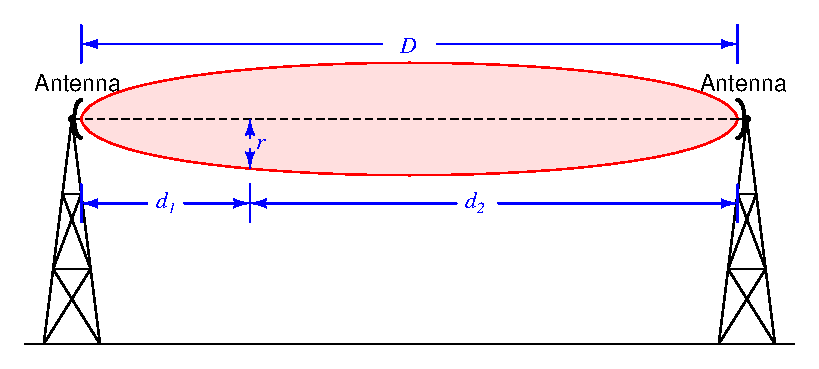
\includegraphics[width=15.5cm]{i01340x01.eps}$$

Skriv denne ligningen om til en form uten de to avstandsmålingene $d_1$ og $d_2$, og erstatt dem med en enkelt variabel $P$ som representerer posisjonen mellom antennene uttrykt som en prosentandel. $P=0\%$ betyr punktet ved venstre antenne, $P=100\%$ betyr punktet ved høyre antenne, og $P=50\%$ betyr punktet nøyaktig halvveis mellom antennene:

$$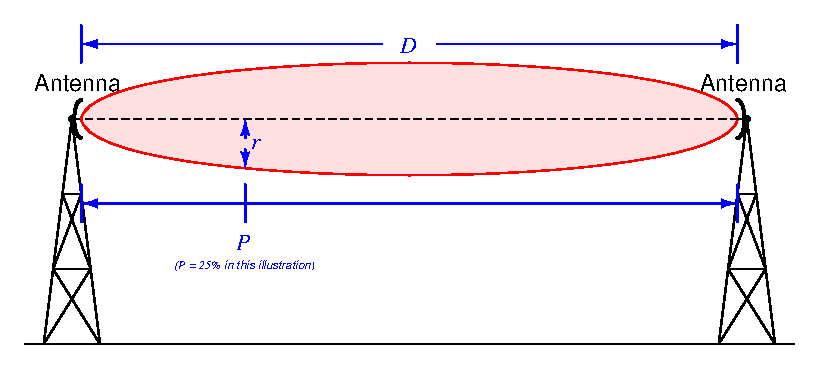
\includegraphics[width=15.5cm]{i01340x02.eps}$$

\vskip 10pt

Tips: $d_1 = PD$

\vskip 10pt

\underbar{file i01340}
%(END_QUESTION)





%(BEGIN_ANSWER)

$$r = \sqrt{{n \lambda PD (D - PD)} \over D}$$

$$\hbox{. . . eller . . .}$$

$$r = \sqrt{n \lambda P D (1 - P)}$$

%(END_ANSWER)





%(BEGIN_NOTES)


%INDEX% Mathematics review: basic principles of algebra
%INDEX% Mathematics review: manipulating and combining equations to form a new equation

%(END_NOTES)
